% Poster Figure 4 (Experimental Setup): character-background separation win rate.
% Data: Tab. sep_multigame in 4_experiments.tex (multi-domain HeroWorld, 48 WASD scenes,
% Gemini-2.5-Pro pairwise judge, k=3 counterbalanced, ties excluded). Sized for a 10.6in x 4.4in slot.
\documentclass[border=2pt]{standalone}
% Shared style for PRISM figures. Compile with tectonic (XeTeX engine).
\usepackage{lmodern}
\usepackage{amssymb}
\usepackage{fontspec}
\setmainfont{Arial}
\setsansfont{Arial}
\usepackage{amsmath}
\usepackage{booktabs}
\usepackage{colortbl}
\usepackage{xcolor}
\usepackage{tikz}
\usetikzlibrary{arrows.meta,positioning,fit,calc,backgrounds,decorations.pathreplacing}
\usepackage{pgfplots}
\pgfplotsset{compat=1.18}

% PRISM template palette (sampled from the poster template)
\definecolor{prismdark}{HTML}{195A99}
\definecolor{prismmid}{HTML}{1D6FAA}
\definecolor{prismlight}{HTML}{9BB7DC}
\definecolor{prismpale}{HTML}{E8EFF8}
\definecolor{prismaccent}{HTML}{D9822B}
\definecolor{prismgray}{HTML}{6B7280}

\newcommand{\sz}[2]{\fontsize{#1}{#2}\selectfont}
\newcommand{\oursrow}{\rowcolor{prismpale}}
\pgfkeys{/pgf/number format/assume math mode=true}

\begin{document}
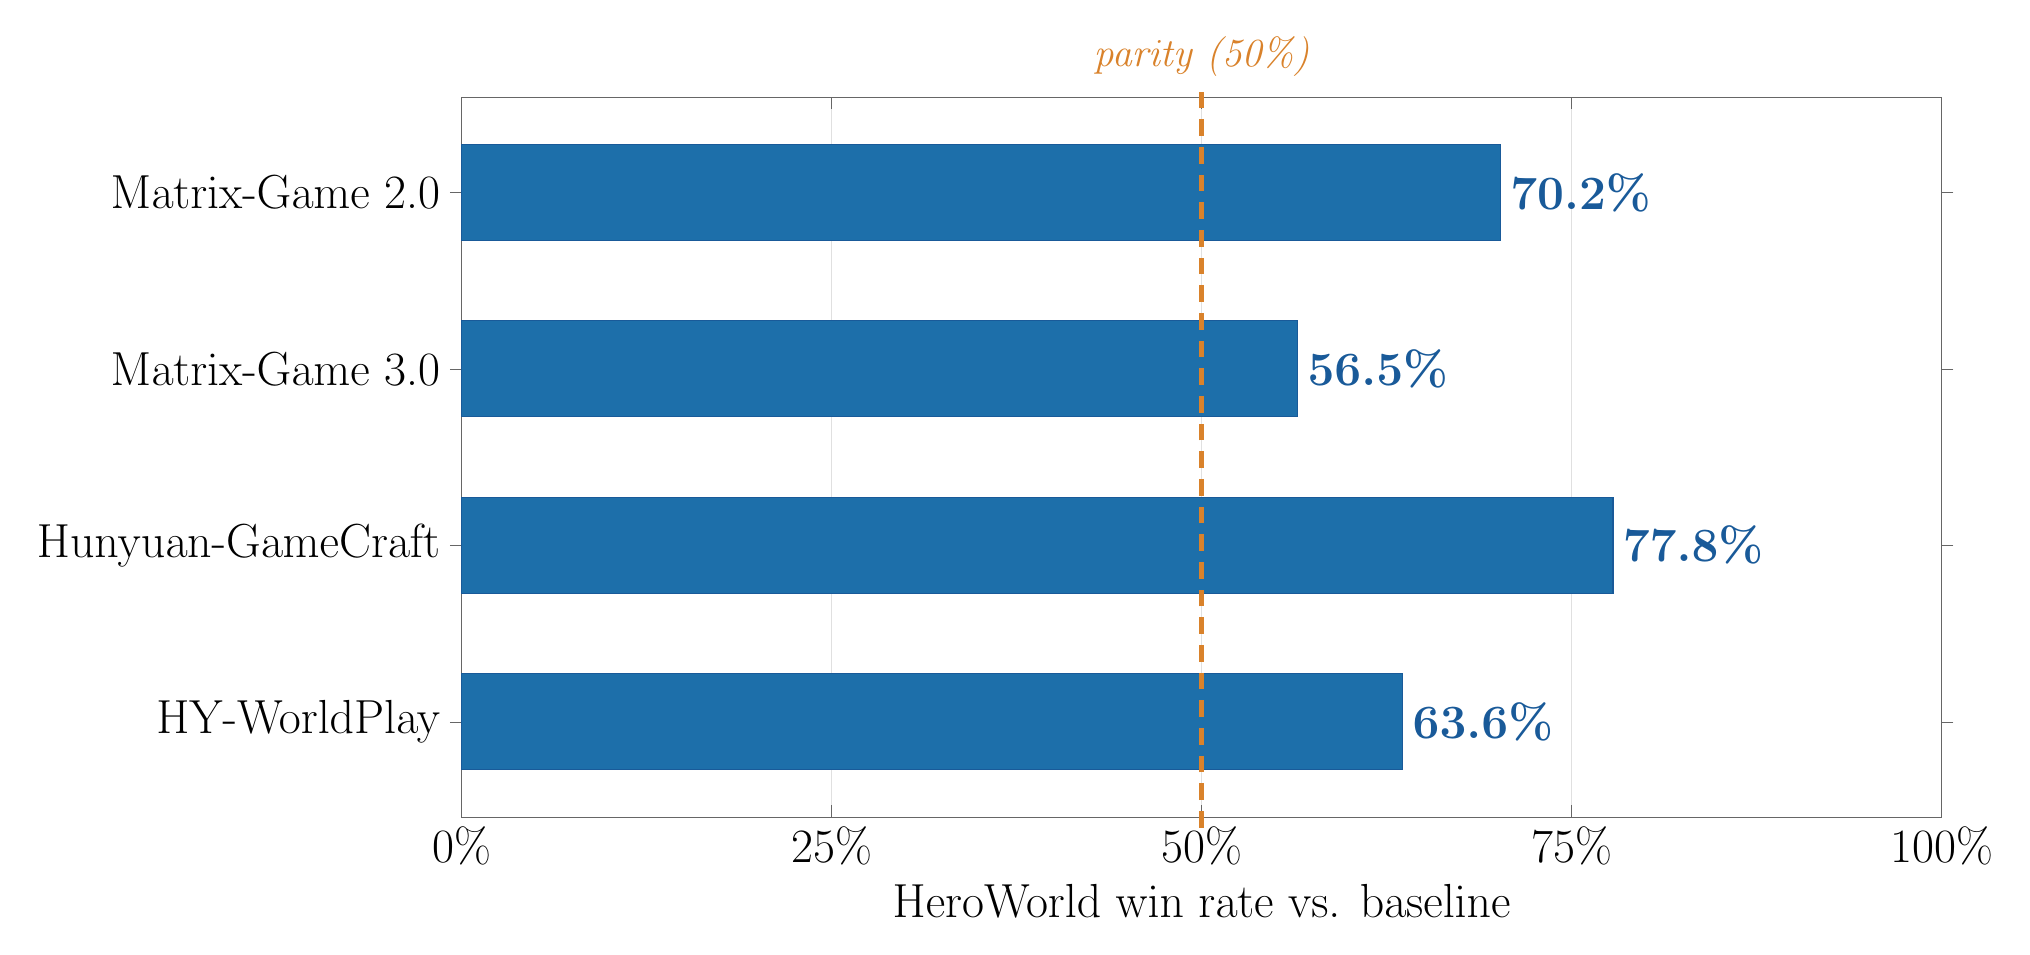
\begin{tikzpicture}
\begin{axis}[
  scale only axis, width=7.4in, height=3.6in,
  xbar, bar width=0.48in,
  xmin=0, xmax=100,
  xtick={0,25,50,75,100}, xticklabel={\pgfmathprintnumber{\tick}\%},
  symbolic y coords={HY-WorldPlay,Hunyuan-GameCraft,Matrix-Game 3.0,Matrix-Game 2.0},
  ytick=data, y dir=normal,
  enlarge y limits=0.18,
  tick label style={font=\sz{17}{20}},
  xlabel={HeroWorld win rate vs. baseline},
  xlabel style={font=\sz{17}{20}},
  axis line style={black!60}, tick style={black!60},
  xmajorgrids, grid style={black!12},
  nodes near coords={\pgfmathprintnumber[fixed,precision=1]{\pgfplotspointmeta}\%},
  nodes near coords style={font=\sz{17}{20}\bfseries, text=prismdark, anchor=west},
  point meta=x,
  clip=false,
]
\addplot[fill=prismmid, draw=prismdark] coordinates {
  (70.2,Matrix-Game 2.0) (56.5,Matrix-Game 3.0) (77.8,Hunyuan-GameCraft) (63.6,HY-WorldPlay)};
\draw[prismaccent, line width=1.6pt, dash pattern=on 6pt off 4pt]
  (axis cs:50,{[normalized]-0.6}) -- (axis cs:50,{[normalized]3.6});
\node[anchor=south, font=\sz{15}{18}\itshape, text=prismaccent] at (axis cs:50,{[normalized]3.6}) {parity (50\%)};
\end{axis}
\end{tikzpicture}
\end{document}
